%% This is an example first chapter.  You should put chapter/appendix that you
%% write into a separate file, and add a line \include{yourfilename} to
%% main.tex, where `yourfilename.tex' is the name of the chapter/appendix file.
%% You can process specific files by typing their names in at the 
%% \files=
%% prompt when you run the file main.tex through LaTeX.
\chapter{Introduction}\label{chapter:intro}

\section{Computer Graphics state and issues}\label{intro:cg}

Computer Graphics is a vast discipline of Computer Sciences. In general, it studies theoretical methods for synthesis of 2-dimensional (2D) images using computers. It also includes research on computer hardware, used for image computing and displaying. Among applications of computer graphics there are: typography, cinema, entertainment, scientific visualization and industrial design. From a physical point of view, the 2D images capture information about how light beams pass through the space and reach our eyes. Then a snapshot of all received light is interpreted by our perception as a sight full of shapes and colors. Images in a computer are usually represented with two major archetypes:

\begin{itemize}
	\item vector images \cite{aux:vector14} - represented by a set of 2D points, lines, polygonal shapes and mathematically defined distribution of color within them;
	\item raster images \cite{aux:raster94} - represented by a uniform rectangular grid (referred to as raster), filled with colored squares (referred to as pixels). Typically, colors are defined using Red-Green-Blue (RGB) color model \cite{aux:color05}, where all possible colors are mixed from 3 primary colors, stored in computers as values in $[0;1]$ range of real numbers (or similarly as values in $[0;255]$ range of integer numbers).
\end{itemize}

Vector graphics is more practical to visualize simple shapes, like schemes or text. It's not much suitable to visualize objects of the real world, as such objects are too complex. They may have arbitrary geometry, specular properties when being illuminated by light or shadowed by other objects. Representing all of that with vector graphics would require hundreds of thousands of unique shapes, which is a lot in terms of computations, human hand-craft, and computer file sizes. 

Although in the raster graphics, the number of pixels may also surpass millions, the structure of pixel grids is uniform, and each pixel stores the same amount of data. Also for most cases, the image data has information redundancy in it, and thus can be compressed \cite{aux:compression18}. Besides, the pixel grid resembles a canvas from the traditional art. Current computer software for creation of raster images has capabilities similar to real brushes and palettes. This intuitive representation allows to speed up production time for humans. And we know that raster images can be very realistic, proven by the visual quality that can be captured with modern digital cameras \cite{aux:camera21}.

Speaking of realism, it's one of the most important challenges in the computer graphics research. The generated images should ideally be indistinguishable from sights we perceive with our own eyes. Unfortunately, the real world is at least 3-dimensional (3D). Thus, it cannot be fully represented with images on a screen or paper, which are 2D by nature. Another obstacle, is that human vision is very sensitive, and it can easily detect unrealistic or anomalous features, e.g. noise, tearing, blurriness and so on. Those are referred to as visual artifacts (also glitches, distortions). However, to this day there haven't been discovered a unified metric of realism, that would allow to compare two similar images and tell which will be more plausible for the human perception \cite{metric:wang11}.

Direct usage of 2D images for visualization of the 3D world isn't always efficient. For example, if we intend to create an animation (a temporarily coherent sequence of images), it would require to draw the same content with slight adjustment between images. Instead of manually copying the content from one image to another and insuring its coherency and synchronization, it's common to instead approximately model the 3D scene of interest. Such scene representations can take explicit forms, e.g. point clouds, voxel grids, triangular meshes, or even implicit functions, such as signed distance fields (SDF)\cite{survey:advances-nn22}\footnote{See Section 3.1. of \cite{survey:advances-nn22}.}\label{intro:3d-representations-paragraph}. After modeling, at every moment of time the geometry's appearance can be projected from a certain view point onto an image. This allows to model the scene one time and reuse it for synthesis of dozens of images.

%A common way to model 3D geometry is triangular meshes \cite{mesh-data-structure}. Here the geometry is defined as a set of 3D vertices and their connectivity into polygons (usually triangles).

Typically 2D images are synthesized from a 3D scene, using rendering algorithms. They emulate the laws of physics that lie within synthesis of images with physical cameras. One such algorithm is \textit{tracing of rays} that travel starting from a light source, bounce from reflective surfaces, until finally they reach an eye or a camera. This method is one of the most photo-realistic, at least to the state of our theoretical understanding of physical specular phenomena. However, it's exceptionally long to compute in great details. That's why a much more coarse algorithm of \textit{rasterization} is typically used, with each simple geometric part of the scene (e.g. points, triangles, voxels) projected onto a 2D image. The color information for each part is extracted from texture images, that capture physical properties of surfaces, such as color, refraction, reflection, etc (see Figure \ref{intro:fig:mesh-texture}). But with either rendering algorithm, there persists a problem that all those properties need to be explicitly specified, often by a human, which drastically increases the difficulty of achieving photo-realism. Besides, some 3D scene representations lack details, some are heavy to be efficiently processed, or require enormous amount of computer storage. In either case, an order of magnitude higher number of geometric details needs to be defined compared to just a 2D image. 

\begin{figure}[h!]
	\centering
	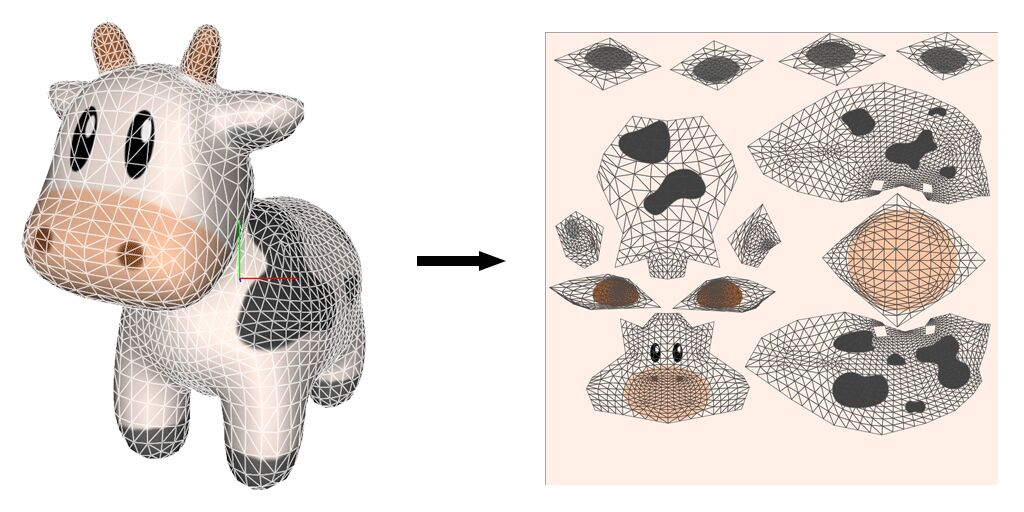
\includegraphics[height=7cm]{\imgfp/mesh-texture}
	\caption{Example of a triangular mesh, with a texture image wrapped on it. Each triangle is mapped to texture coordinates, that in turn allow to sample a color patch on the texture. A rasteriazation process projects every triangle onto an image, and interpolates texture coordinates for every image pixel, to then sample corresponding color values from the texture. Picture source: \href{https://metalbyexample.com/textures-and-samplers/}{metalbyexample.com/textures-and-samplers}}
	\label{intro:fig:mesh-texture}
\end{figure}


\section{Neural Rendering}\label{intro:nrender}

In the last decades, the methods of Artificial Intelligence (AI) and its sub-fields of Machine Learning (ML) and Deep Neural Networks (DNN) have emerged to solve multidisciplinary problems of science and business. Instead of modeling a phenomenon algorithmically, they aim to approximate statistical properties of data captured from the phenomenon. Generally, input data is passed down a highly-parameterized computational graph, and output is compared to certain desired data. During a process referred to as a optimization (training, tuning), the parameters of the graph are iteratively adjusted to better fit the desired data. Afterwards, the computational graph is expected to be general enough to also accurately model the data, that was never seen during training. The automation is what makes these approaches groundbreaking. Unlike humans, numerical algorithms can capture very complex statistical correlations or patterns in highly-dimensional data, including images.

A selection of computer graphics problems may also be solved by means of ML and DNN methods. A few notable research topics in this field include:
\begin{itemize}
\item image impainting -- completion of missing parts on an image with semantically fitting content;
\item image super-resolution -- up-scaling an image and making it more detailed;
\item reconstruction of 3D objects -- automated creation of an object's 3D representation (see page \pageref{intro:3d-representations-paragraph}) and materials from 2D images captured with physical cameras;
\item neural rendering -- automated synthesis of realistic images with certain expected content.
\end{itemize}

This thesis focuses on the topic of neural rendering, although its definition is quite vague. A default approach is to use traditional algorithms to generate a simple image that describes coarse information about a scene, such as general outlines of each separate object, distance from a camera, etc. Then an AI model is used to generate the final image -- realistic, detailed, possibly with higher resolution \cite{dnn:deferred19}. There's another branch of research, where the AI is used to represent the 3D scene, often implicitly as weights of the AI model. Then this representation is decoded (sampled) into 2D images using deterministic algorithms \cite{dnn:nerf20}.
 
It's very rare to have a detailed, realistic and diverse dataset of 3D scenes that we want to reconstruct with neural rendering. Instead, AI models are typically trained on physical camera images, thus combining tasks of 3D object reconstruction and neural rendering. It's known to be a very tough challenge for man-made algorithms, and not as much easier for AI models. On the other hand, there already exist solutions that may surpass any manual human labor on image synthesis or scene modeling \cite{dnn:stylegan-v1-19,dnn:stylegan-v2-20,dnn:stylegan-v3-21,dnn:nerf20}.
 
However, training an AI model for generating photo-realistic images is only a half of the challenge. Every AI model is meant to be integrated into a real application and executed (inferred) on some computing device. It can be a stationary computer with lots of computing power. It can also be mobile hardware, since in the last years their computing power became powerful enough to infer AI models in real-time. Such hardware is included in modern smartphones, Augmented Reality (AR), or Virtual Reality (VR) head mounted displays. Running DNN models here directly provides lower latency of computations, better privacy and data security. But also, many performance, compute and power usage constraints may arise:
\begin{itemize}
	\item  AI models that run in real-time applications need to deliver results multiple times per second.
	\item  The computing resources are limited due to a small physical size of the hardware. Resources are even further restricted, in order to reduce overheat and to improve battery life.
	\item  AI models that utilize customer devices by any means need to deal with compatibility issues (e.g. between operating systems, computing architectures, memory layouts).
\end{itemize}

This makes real usage of AI models a very challenging task. AI projects have to rely on standardized software and hardware solutions, that allow easier integration of new AI advancements. However, a unified way to efficiently run arbitrary AI models on every hardware is absent. It's often, that instead a particular AI architecture is manually integrated for a particular type of hardware, squeezing the maximum performance out of them. This is the main way-out for the current projects to obtain any business value from combining state-of-the-art hardware and AI.
 
\section{Project tasks}\label{intro:task}
 
Samsung AI Center at Moscow had been researching on real-time neural rendering of human avatar images. Their recent DNN architecture \cite{dnn:stylepeople21} takes as an input a rasterized image with a body mesh with absent clothing, hair and distinctive person features. When trained with high image resolution, this architecture has proven to fill in those details on the image, producing good full-body (FB) images with a single person. However, the performance concerns for real time avatar rendering weren't profoundly researched.
 
%The model is trained to model appearance of a single person, captured as a 1-2 minute video from a smartphone camera. The distinctive features are learned into a neural texture, which wraps the triangular mesh, and interpretable by the DNN only to model clothes, skin, hair and facial features. 

During the Skoltech's Summer Immersion of Master students in 2021, a development of a mobile Android application was started from scratch. It needs to serve as a test of performance, visual quality and compatibility of the aforementioned architecture on mobile devices. The application should prepare input data for the DNN and visualize avatar images on top of camera frames as AR, i.e. as if images are part of the captured environment. Camera movements allow to observe the avatar from arbitrary distance and angle.
 
The main concern is to obtain a balance of performance and visual quality of the mobile AR application. For instance, with the minimal acceptable avatar resolution of $512\times512$ pixels, the performance of the researched DNNs is too low. Each frame computing takes more than 60 milliseconds (ms) on the most recent modern mobile hardware (Qualcomm Snapdragon 888). However, a computation time lower than 33ms per frame is required for smooth AR experience, which is equivalent to more than 30 frames per second (FPS). Moreover, the architecture's training process could be adjusted with AR usage in mind. For example, when we move camera close to the avatar, effectively only a small part of the body can be seen by the user. But if the DNN generates full body images regardless, a big part of computations is wasted. And the seen part will be in a fairly low resolution. When rendered on a mobile screen with high resolution, it appears as a very ``pixelated'' image in low details (see Figure \ref{intro:fig:stylepeople_frame}\protect\subref{intro:fig:stylepeople_frame:waste}). Also the DNN should be stable in views that are possible in AR, but not present in the training data, e.g. straight top-down or bottom-up views. 

\begin{figure}[h!]
	\fboxrule=2pt
	\centering
	\begin{subfigure}[b]{0.4\textwidth}
		\centering
		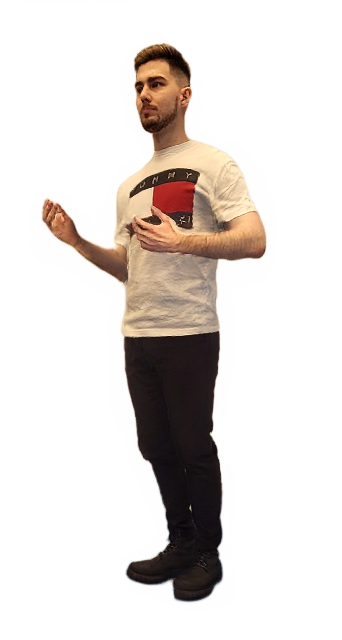
\includegraphics[height=10cm]{\imgfp/frame_640_narrow}
		\caption{}
		\label{intro:fig:stylepeople_frame:640}
	\end{subfigure}
	\hfill
	\begin{subfigure}[b]{0.59\textwidth}
		\centering
		
\includegraphics[height=10cm]{\imgfp/frame_waste}
		\caption{}
		\label{intro:fig:stylepeople_frame:waste}
	\end{subfigure}

	\caption{(\protect\subref{intro:fig:stylepeople_frame:640}) A full-body image generated with the baseline DNN \cite{dnn:stylepeople21}. (\protect\subref{intro:fig:stylepeople_frame:waste}) Full body image synthesis for AR, but only a small image part is visible and in low resolution, the rest is wasted.}
	\label{intro:fig:stylepeople_frame}
\end{figure}
 
The goal of this thesis is to continue the aforementioned project. The first high-level task is to achieve an admissible trade off of performance and visual quality, when executing the DNN as a part of mobile AR experience. Target devices are the latest mobile phones running on Qualcomm Snapdragon System on the Chip (SoC), with Android operating system. The second task is to research on adjusting DNN training to produce better quality images on zoomed scales (upper body, close-up), while retaining similar quality in full-body scale. However, it's advisable to keep the same baseline \cite{dnn:stylepeople21} DNN architecture if possible, because integration of a completely new pipeline may contradict the implementation of the first task, and will require significant time on obtaining better results and integration.
 
The specific tasks are defined in details as follows:
\begin{enumerate}
	\item To implement real-time input generation on mobile, for the baseline DNNs. This includes inference of a posed mesh of a unified human body model \cite{dnn:smplx19}, extraction of camera tracking information, mesh rasterization as a 2D image, its passing to the DNN running on mobile.
	\item To research on decreasing inference time of the baseline \cite{dnn:stylepeople21} DNN architecture on mobile. It should be possible to infer it with real-time performance of at least 30 FPS, and resolution of the generated images above $256\times256$ pixels.
	\item To research on DNN's training improvements, to make it robust to out-of-distribution views. For example, extremely far zooms, extremely close zooms, rotations and angles of view, while preserving full-body quality.
	\item To achieve execution of the DNNs on specialized mobile hardware for fast quantized AI computations (see Section \ref{lit:mobile}). To compare visual difference between outputs of the default model and outputs on mobile.
	\item To research on algorithmic improvements that would compensate weaknesses of plain DNN's inference, improving either performance or visual quality of avatars.

\end{enumerate}

\newpage

%\section{Motivations for micro-optimization}


%\section{Description of micro-optimization}\label{ch1:opts}

%In order to perform a sequence of floating point operations, a normal FPU
%performs many redundant internal shifts and normalizations in the process of
%performing a sequence of operations.  However, if a compiler can
%decompose the floating point operations it needs down to the lowest level,
%it then can optimize away many of these redundant operations.  
%
%If there is some additional hardware support specifically for
%micro-optimization, there are additional optimizations that can be
%performed.  This hardware support entails extra ``guard bits'' on the
%standard floating point formats, to allow several unnormalized operations to
%be performed in a row without the loss information\footnote{A description of
%	the floating point format used is shown in figures~\ref{exponent-format}
%	and~\ref{mantissa-format}.}.  A discussion of the mathematics behind
%unnormalized arithmetic is in appendix~\ref{unnorm-math}.
%
%The optimizations that the compiler can perform fall into several categories:
%
%\subsection{Post Multiply Normalization}
%
%When more than two multiplications are performed in a row, the intermediate
%normalization of the results between multiplications can be eliminated.
%This is because with each multiplication, the mantissa can become
%denormalized by at most one bit.  If there are guard bits on the mantissas
%to prevent bits from ``falling off'' the end during multiplications, the
%normalization can be postponed until after a sequence of several
%multiplies\footnote{Using unnormalized numbers for math is not a new idea; a
%	good example of it is the Control Data CDC 6600, designed by Seymour Cray.
%	\cite{knuthwebsite} The CDC 6600 had all of its instructions performing
%	unnormalized arithmetic, with a separate {\tt NORMALIZE} instruction.}.
%
%% This is an example of how you would use tgrind to include an example
%% of source code; it is commented out in this template since the code
%% example file does not exist.  To use it, you need to remove the '%' on the
%% beginning of the line, and insert your own information in the call.
%%
%%\tagrind[htbp]{code/pmn.s.tex}{Post Multiply Normalization}{opt:pmn}
%
%As you can see, the intermediate results can be multiplied together, with no
%need for intermediate normalizations due to the guard bit.  It is only at
%the end of the operation that the normalization must be performed, in order
%to get it into a format suitable for storing in memory\footnote{Note that
%	for purposed of clarity, the pipeline delays were considered to be 0, and
%	the branches were not delayed.}.
%
%\subsection{Block Exponent}
%
%In a unoptimized sequence of additions, the sequence of operations is as
%follows for each pair of numbers ($m_1$,$e_1$) and ($m_2$,$e_2$).
%\begin{enumerate}
%	\item Compare $e_1$ and $e_2$.
%	\item Shift the mantissa associated with the smaller exponent $|e_1-e_2|$
%	places to the right.
%	\item Add $m_1$ and $m_2$.
%	\item Find the first one in the resulting mantissa.
%	\item Shift the resulting mantissa so that normalized
%	\item Adjust the exponent accordingly.
%\end{enumerate}
%
%Out of 6 steps, only one is the actual addition, and the rest are involved
%in aligning the mantissas prior to the add, and then normalizing the result
%afterward.  In the block exponent optimization, the largest mantissa is
%found to start with, and all the mantissa's shifted before any additions
%take place.  Once the mantissas have been shifted, the additions can take
%place one after another\footnote{This requires that for n consecutive
%	additions, there are $\log_{2}n$ high guard bits to prevent overflow.  In
%	the $\mu$FPU, there are 3 guard bits, making up to 8 consecutive additions
%	possible.}.  An example of the Block Exponent optimization on the expression
%X = A + B + C is given in figure~\ref{opt:be}.
%
%% This is an example of how you would use tgrind to include an example
%% of source code; it is commented out in this template since the code
%% example file does not exist.  To use it, you need to remove the '%' on the
%% beginning of the line, and insert your own information in the call.
%%
%%\tgrind[htbp]{code/be.s.tex}{Block Exponent}{opt:be}
%
%\section{Integer optimizations}
%
%As well as the floating point optimizations described above, there are
%also integer optimizations that can be used in the $\mu$FPU.  In concert
%with the floating point optimizations, these can provide a significant
%speedup.  
%
%\subsection{Conversion to fixed point}
%
%Integer operations are much faster than floating point operations; if it is
%possible to replace floating point operations with fixed point operations,
%this would provide a significant increase in speed.
%
%This conversion can either take place automatically or or based on a
%specific request from the programmer.  To do this automatically, the
%compiler must either be very smart, or play fast and loose with the accuracy
%and precision of the programmer's variables.  To be ``smart'', the computer
%must track the ranges of all the floating point variables through the
%program, and then see if there are any potential candidates for conversion
%to floating point.  This technique is discussed further in
%section~\ref{range-tracking}, where it was implemented.
%
%The other way to do this is to rely on specific hints from the programmer
%that a certain value will only assume a specific range, and that only a
%specific precision is desired.  This is somewhat more taxing on the
%programmer, in that he has to know the ranges that his values will take at
%declaration time (something normally abstracted away), but it does provide
%the opportunity for fine-tuning already working code.
%
%Potential applications of this would be simulation programs, where the
%variable represents some physical quantity; the constraints of the physical
%system may provide bounds on the range the variable can take.
%\subsection{Small Constant Multiplications}
%
%One other class of optimizations that can be done is to replace
%multiplications by small integer constants into some combination of
%additions and shifts.  Addition and shifting can be significantly faster
%than multiplication.  This is done by using some combination of
%\begin{eqnarray*}
%	a_i & = & a_j + a_k \\
%	a_i & = & 2a_j + a_k \\
%	a_i & = & 4a_j + a_k \\
%	a_i & = & 8a_j + a_k \\
%	a_i & = & a_j - a_k \\
%	a_i & = & a_j \ll m \mbox{shift}
%\end{eqnarray*}
%instead of the multiplication.  For example, to multiply $s$ by 10 and store
%the result in $r$, you could use:
%\begin{eqnarray*}
%	r & = & 4s + s\\
%	r & = & r + r
%\end{eqnarray*}
%Or by 59:
%\begin{eqnarray*}
%	t & = & 2s + s \\
%	r & = & 2t + s \\
%	r & = & 8r + t
%\end{eqnarray*}
%Similar combinations can be found for almost all of the smaller
%integers\footnote{This optimization is only an ``optimization'', of course,
%	when the amount of time spent on the shifts and adds is less than the time
%	that would be spent doing the multiplication.  Since the time costs of these
%	operations are known to the compiler in order for it to do scheduling, it is
%	easy for the compiler to determine when this optimization is worth using.}.
%\cite{einstein}
%
%\section{Other optimizations}
%
%\subsection{Low-level parallelism}
%
%The current trend is towards duplicating hardware at the lowest level to
%provide parallelism\footnote{This can been seen in the i860; floating point
%	additions and multiplications can proceed at the same time, and the RISC
%	core be moving data in and out of the floating point registers and providing
%	flow control at the same time the floating point units are active. \cite{knuthwebsite}}
%
%Conceptually, it is easy to take advantage to low-level parallelism in the
%instruction stream by simply adding more functional units to the $\mu$FPU,
%widening the instruction word to control them, and then scheduling as many
%operations to take place at one time as possible.
%
%However, simply adding more functional units can only be done so many times;
%there is only a limited amount of parallelism directly available in the
%instruction stream, and without it, much of the extra resources will go to
%waste.  One process used to make more instructions potentially schedulable
%at any given time is ``trace scheduling''.  This technique originated in the
%Bulldog compiler for the original VLIW machine, the ELI-512.
%\cite{latexcompanion,einstein}  In trace scheduling, code can be
%scheduled through many basic blocks at one time, following a single
%potential ``trace'' of program execution.  In this way, instructions that
%{\em might\/} be executed depending on a conditional branch further down in
%the instruction stream are scheduled, allowing an increase in the potential
%parallelism.  To account for the cases where the expected branch wasn't
%taken, correction code is inserted after the branches to undo the effects of
%any prematurely executed instructions.
%
%\subsection{Pipeline optimizations}
%
%In addition to having operations going on in parallel across functional
%units, it is also typical to have several operations in various stages of
%completion in each unit.  This pipelining allows the throughput of the
%functional units to be increased, with no increase in latency.
%
%There are several ways pipelined operations can be optimized.  On the
%hardware side, support can be added to allow data to be recirculated back
%into the beginning of the pipeline from the end, saving a trip through the
%registers.  On the software side, the compiler can utilize several tricks to
%try to fill up as many of the pipeline delay slots as possible, as
%seendescribed by Gibbons. \cite{knuthwebsite}


